\begin{frame}
  \frametitle{New features in the past few months - June 2026}

    \vspace{-2em}


    \begin{center}
    \begin{tikzpicture}[
        stat/.style={
            draw,
            rounded corners,
            minimum width=3.2cm,
            minimum height=1.8cm,
            align=center,
            fill=structure.fg,
            text=white
        },
    ]

    \node[stat] (r1) {
        {\Huge\bfseries 16}\\[-0.2em]
        {\scriptsize Releases}
    };

    \node[stat, right=0.5cm of r1] (r2) {
        {\Huge\bfseries 2851}\\[-0.2em]
        {\scriptsize Total Commits}
    };

    \node[stat, right=0.5cm of r2] (r3) {
        {\Huge\bfseries 167}\\[-0.2em]
        {\scriptsize Pull Requests}
    };

    \node[stat, right=0.5cm of r3] (r4) {
        {\Huge\bfseries 72}\\[-0.2em]
        {\scriptsize Contributors}
    };

    \end{tikzpicture}

    \vspace{1.0em}

    \begin{tikzpicture}[
        stat/.style={
            draw,
            rounded corners,
            minimum width=3.2cm,
            minimum height=1.8cm,
            align=center,
            fill=structure.fg,
            text=white
        }
    ]

    \node[
        draw,
        rounded corners,
        minimum width=14.4cm,
        minimum height=1.2cm,
        align=center,
        fill=structure.fg,
        text=white
    ] (detail) {
        \small
        \textbf{1619} commits on MISP core
        \hspace{1em}$\bullet$\hspace{1em}
        \textbf{1232} commits across 18 modules
        \hspace{1em}$\bullet$\hspace{1em}
        \textbf{145} merged pull requests
    };

    \end{tikzpicture}
    \end{center}

    % \vspace{1.0em}

    \begin{itemize}
        \item {\bf UI/UX modernisation}
        \item New {\bf dashboard} system
        \item New {\bf event templating} system
        \item {\bf Geolocation \& map} visualisation
        \item \textbf{Continuous Security Hardening} --- \alert{Regular updates remain critical}
    \end{itemize}

\end{frame}


\begin{frame}
    \frametitle{UI/UX modernisation}

    \vspace{-4em}
    \alertbox{info}{The biggest visual change in years!}{}
    \vspace{-0.3em}

    \begin{itemize}
        \item {\bf Theme system} --- opt-in themes let users preview new UIs
        \begin{itemize}
            \item {\bf BetaUI} --- a community-contributed UX rework (Chris Horsley, Cosive)
                \begin{itemize}
                    \item[] A redesigned, responsive event index \& reorganised navigation
                \end{itemize}
            \item {\bf Overmind} --- the next-generation interface
                \begin{itemize}
                    \item[] Refreshed look and new views
                \end{itemize}
        \end{itemize}
        \item {\bf Decomposed event view} --- the monolithic event view split into specialized views
        \item {\bf Modern front-end stack} Migrating MISP to {\bf Bootstrap 5} and {\bf Font Awesome 7}
    \end{itemize}

\end{frame}

\begin{frame}
    \frametitle{UI/UX modernisation}

    \begin{center}

    \begin{minipage}[t]{0.43\textwidth}
        \centering
        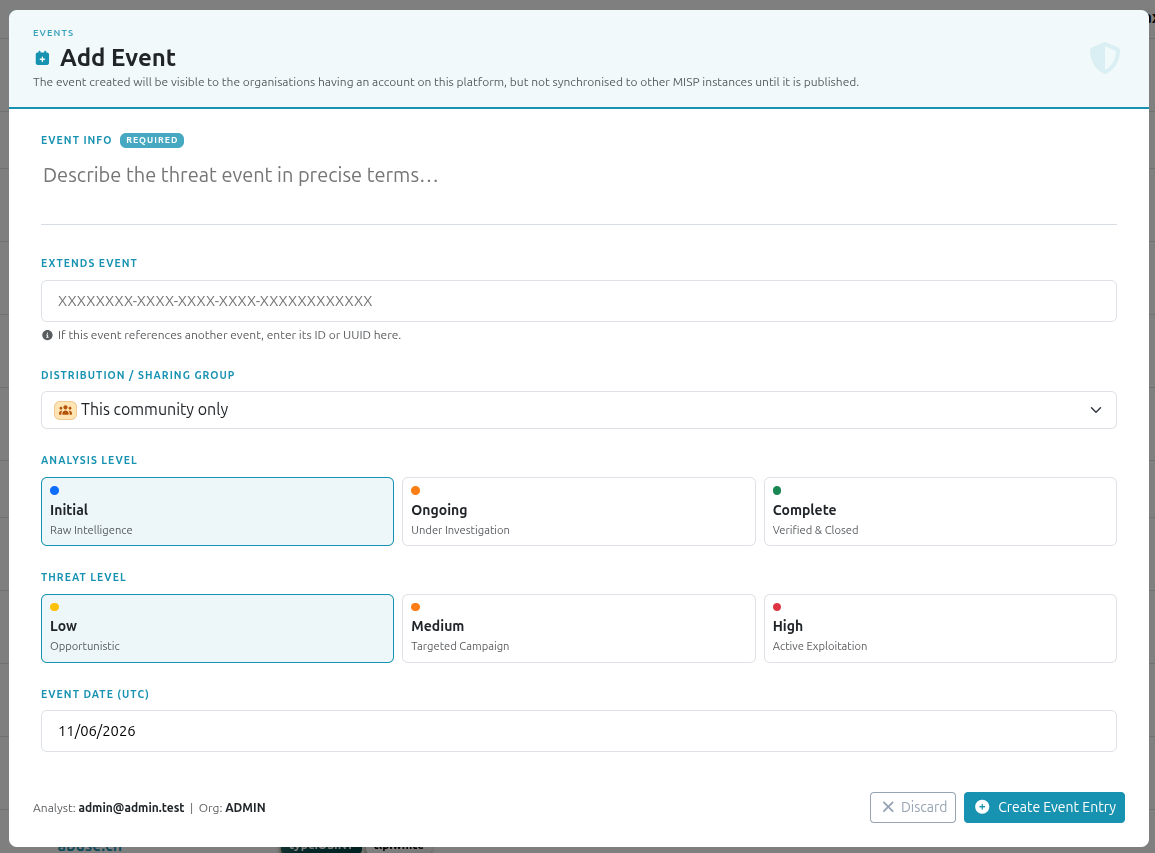
\includegraphics[width=\linewidth, height=0.32\textheight, keepaspectratio]{./img/event-add}

        \vspace{0.3em}
        \scriptsize \texttt{/event/add}
    \end{minipage}
    \hfill
    \begin{minipage}[t]{0.55\textwidth}
        \centering
        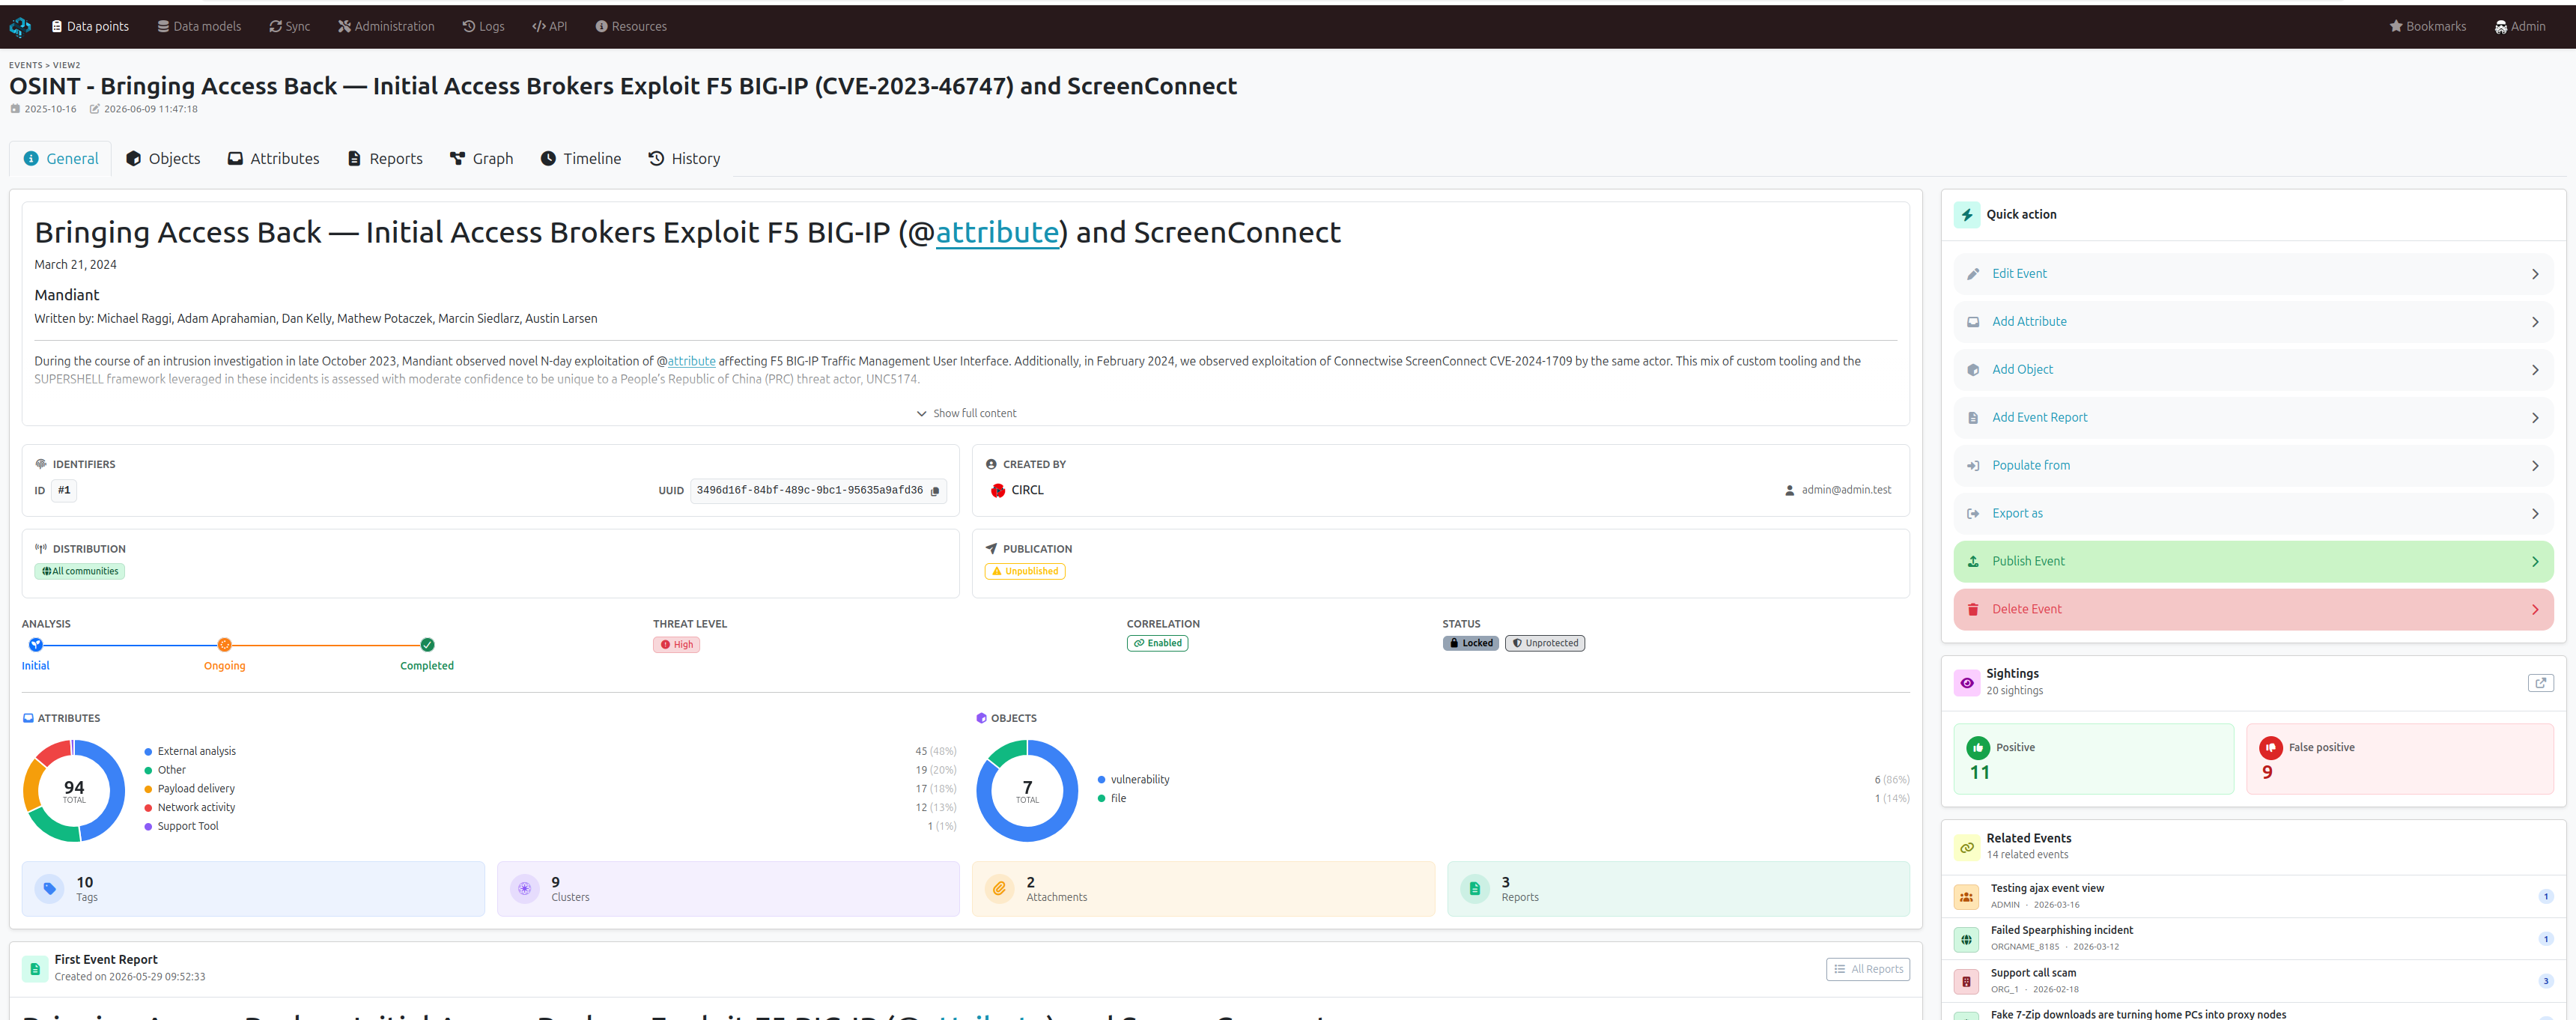
\includegraphics[width=\linewidth, height=0.32\textheight, keepaspectratio]{./img/event-overmind}

        \vspace{0.1em}
        \scriptsize \texttt{/event/view}
    \end{minipage}

    \vspace{0.5em}

    \begin{minipage}[t]{0.48\textwidth}
        \centering
        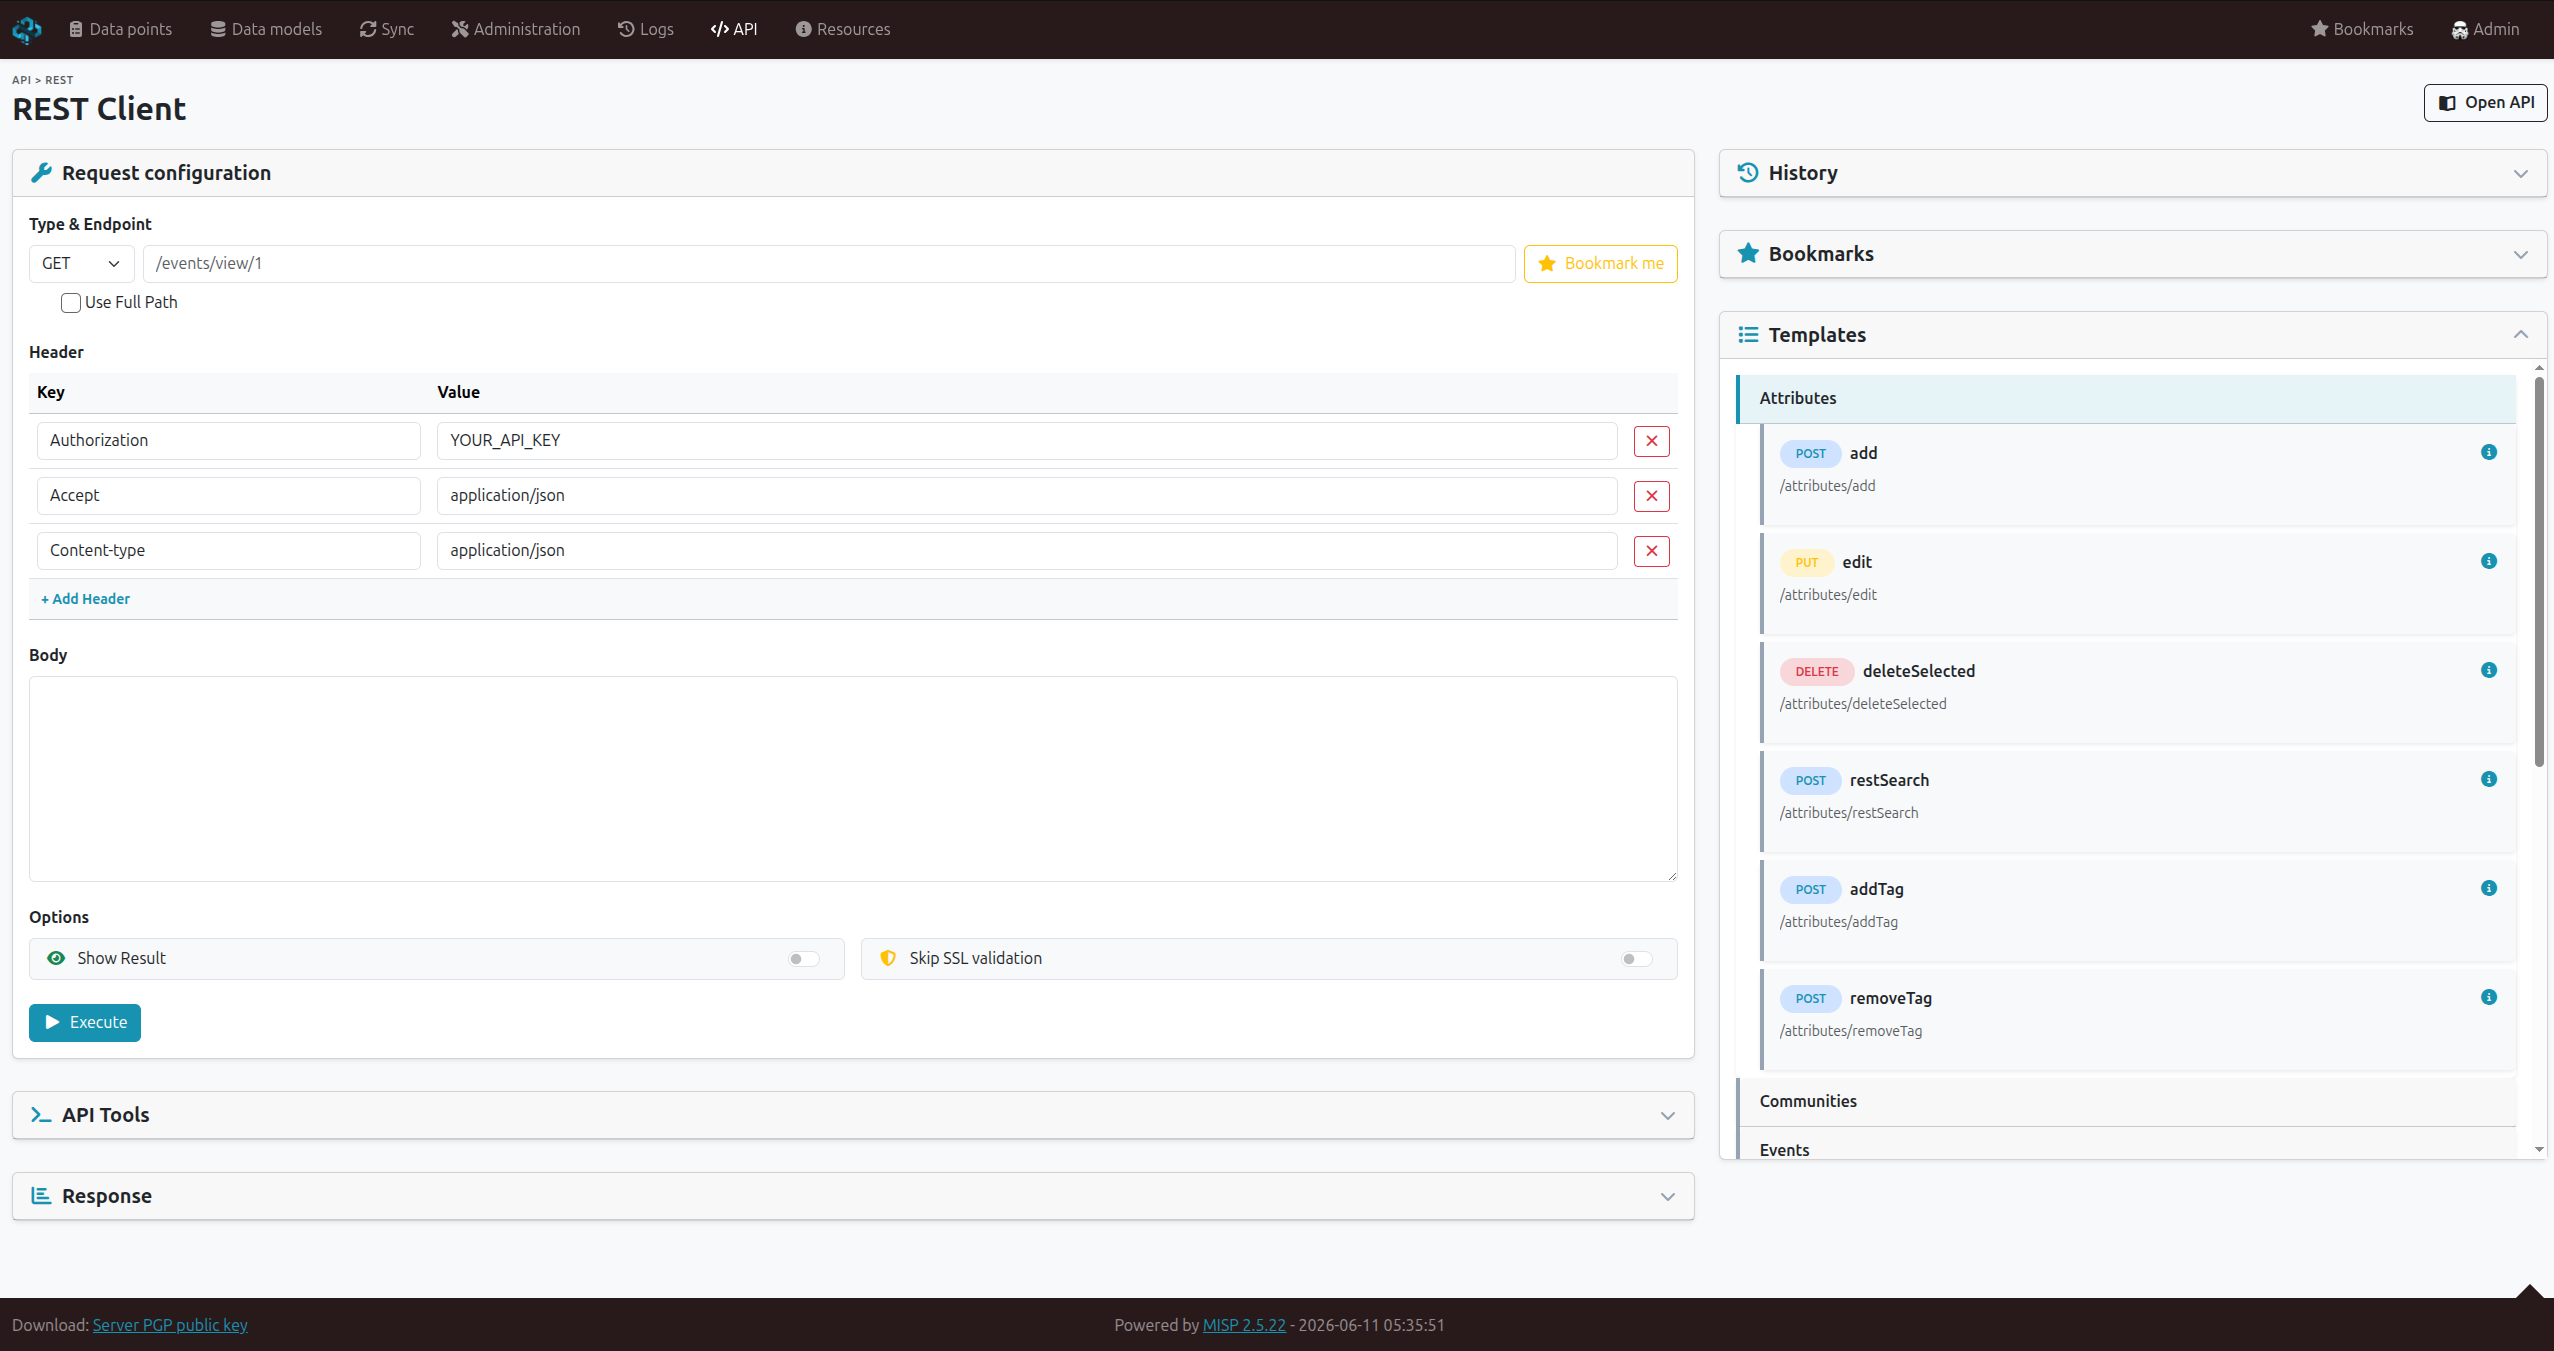
\includegraphics[width=\linewidth, height=0.32\textheight, keepaspectratio]{./img/rest-client.png}

        \vspace{0.3em}
        \scriptsize \texttt{/api/rest}
    \end{minipage}
    \hfill
    \begin{minipage}[t]{0.48\textwidth}
        \centering
        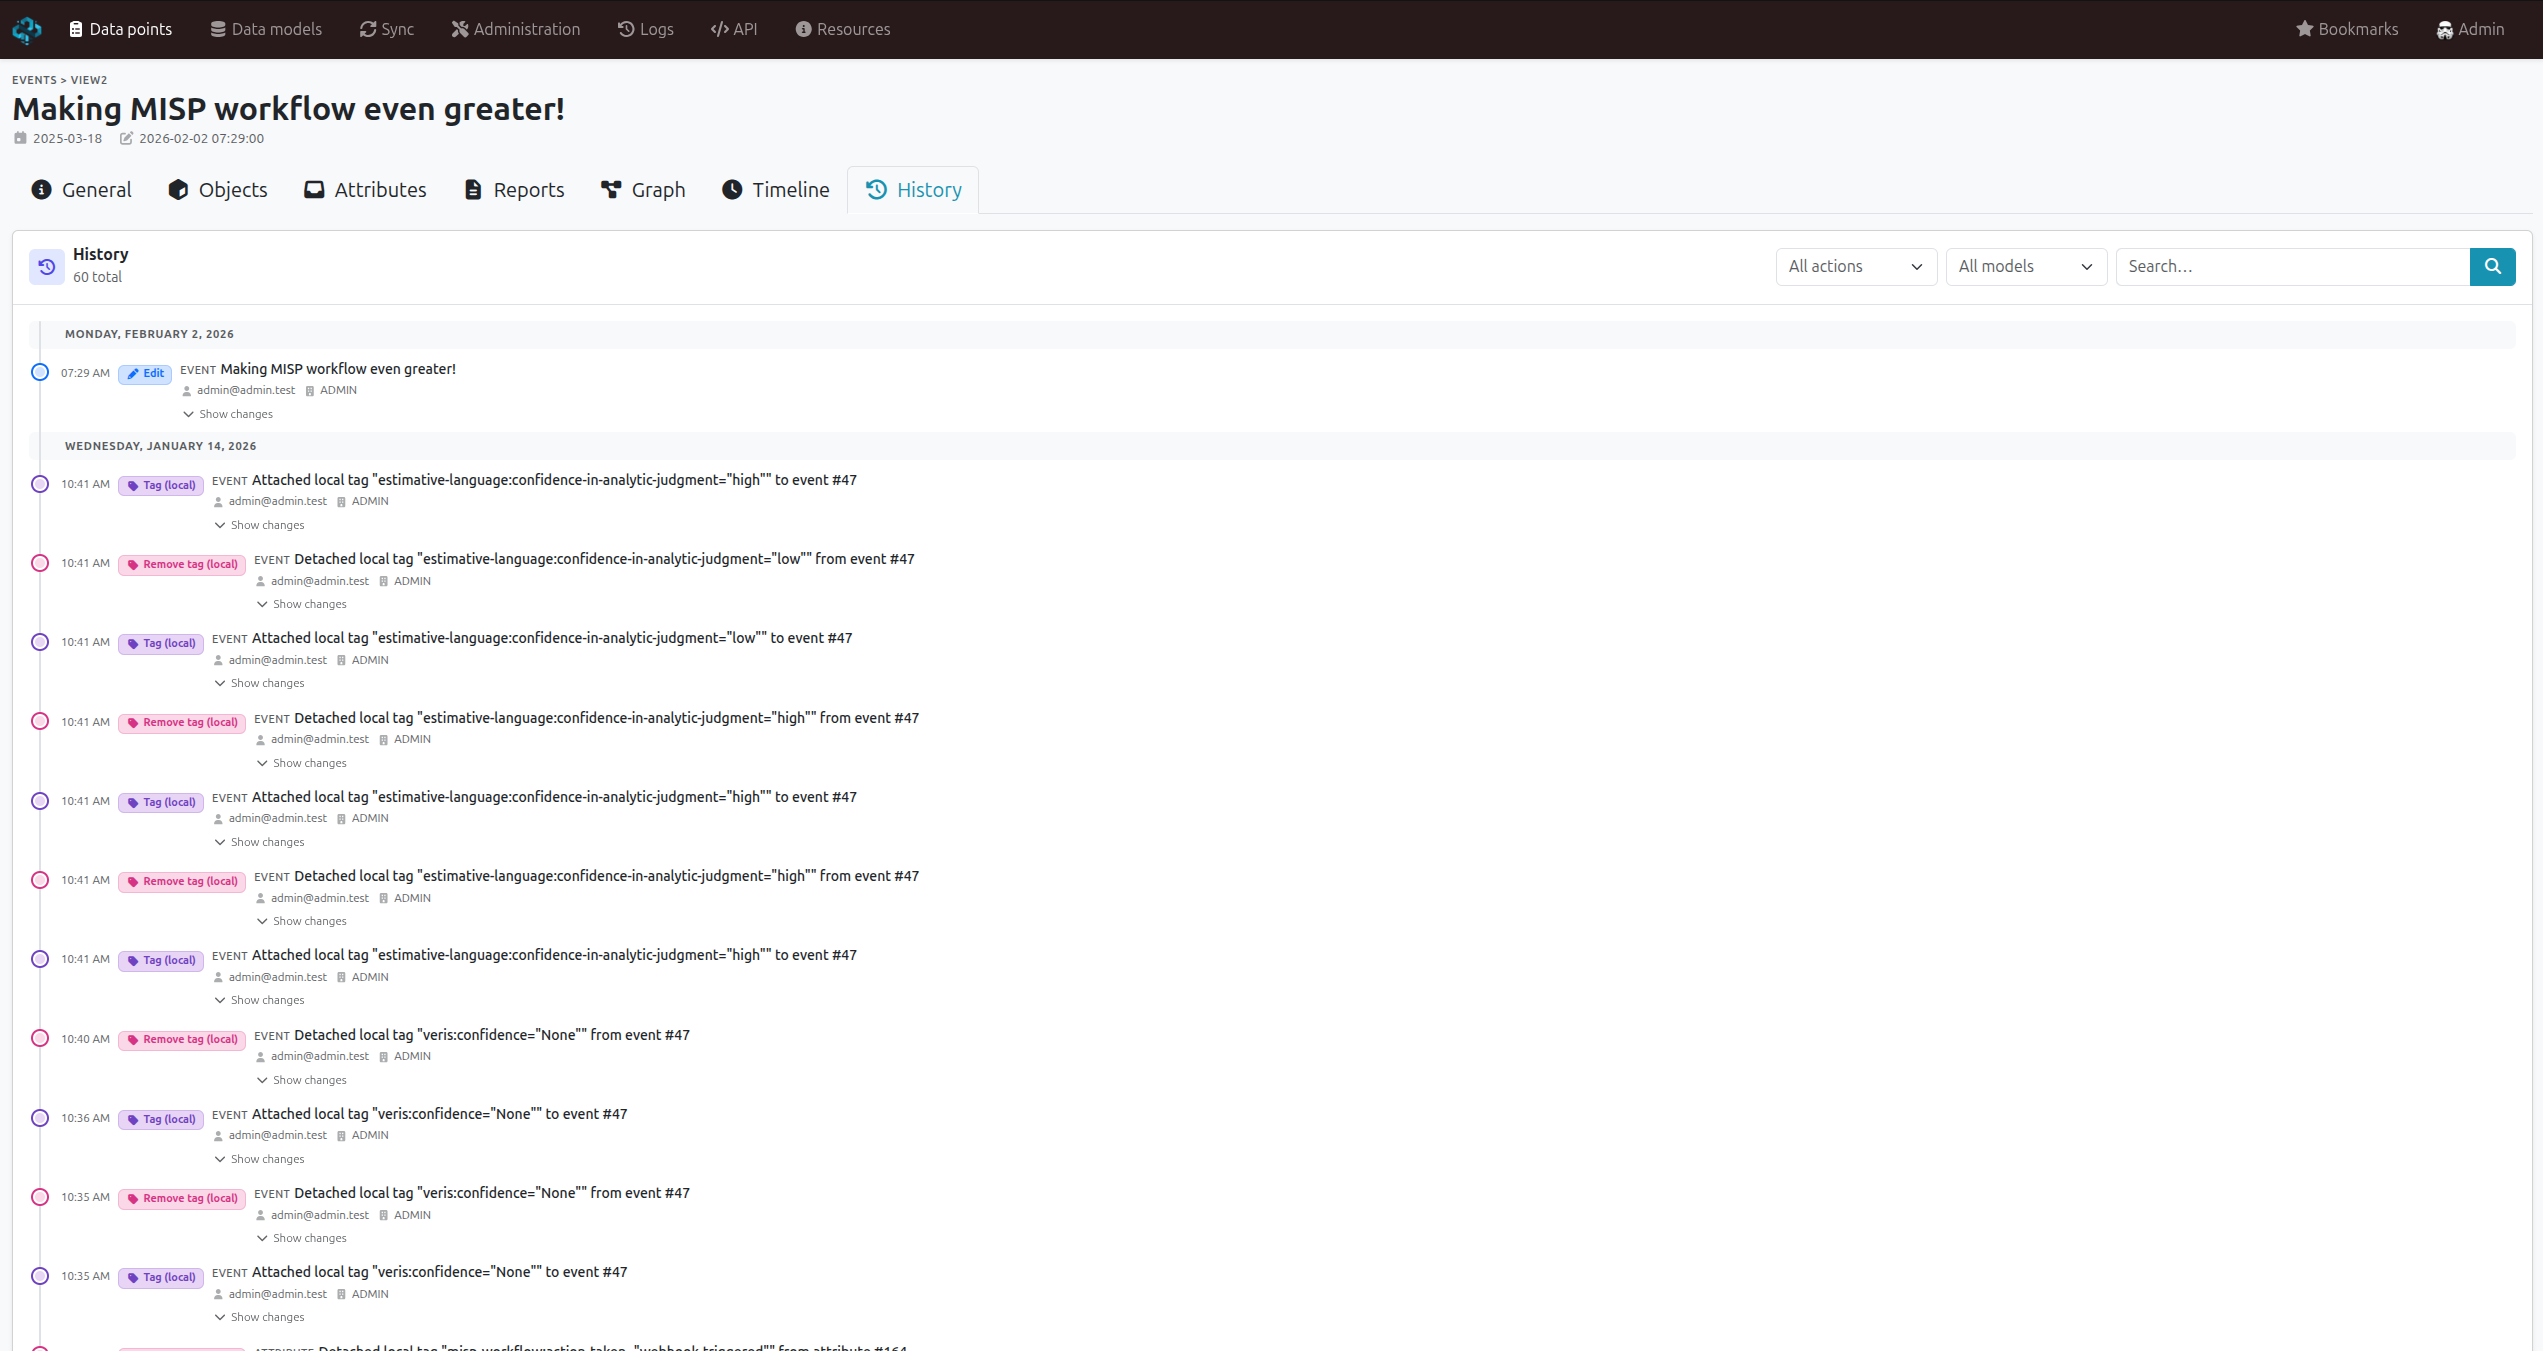
\includegraphics[width=\linewidth, height=0.32\textheight, keepaspectratio]{./img/event-view-history.png}

        \vspace{0.3em}
        \scriptsize \texttt{/event/view-history}
    \end{minipage}

    \end{center}

\end{frame}


\begin{frame}
    \frametitle{New dashboard system}

    \begin{itemize}
        \item A redesign of the MISP dashboard
        \item {\bf Widget gallery} for discovering and adding widgets, with on-demand thumbnails
        \item Richer {\bf chart-based widgets}
        \item Full UI support of parameters and {\bf global dashboard filters}
        \item Foundation for {\bf analyst-focused dashboards} and per-organisation views
    \end{itemize}

\end{frame}


\begin{frame}
    \frametitle{New dashboard system}

    \centering
    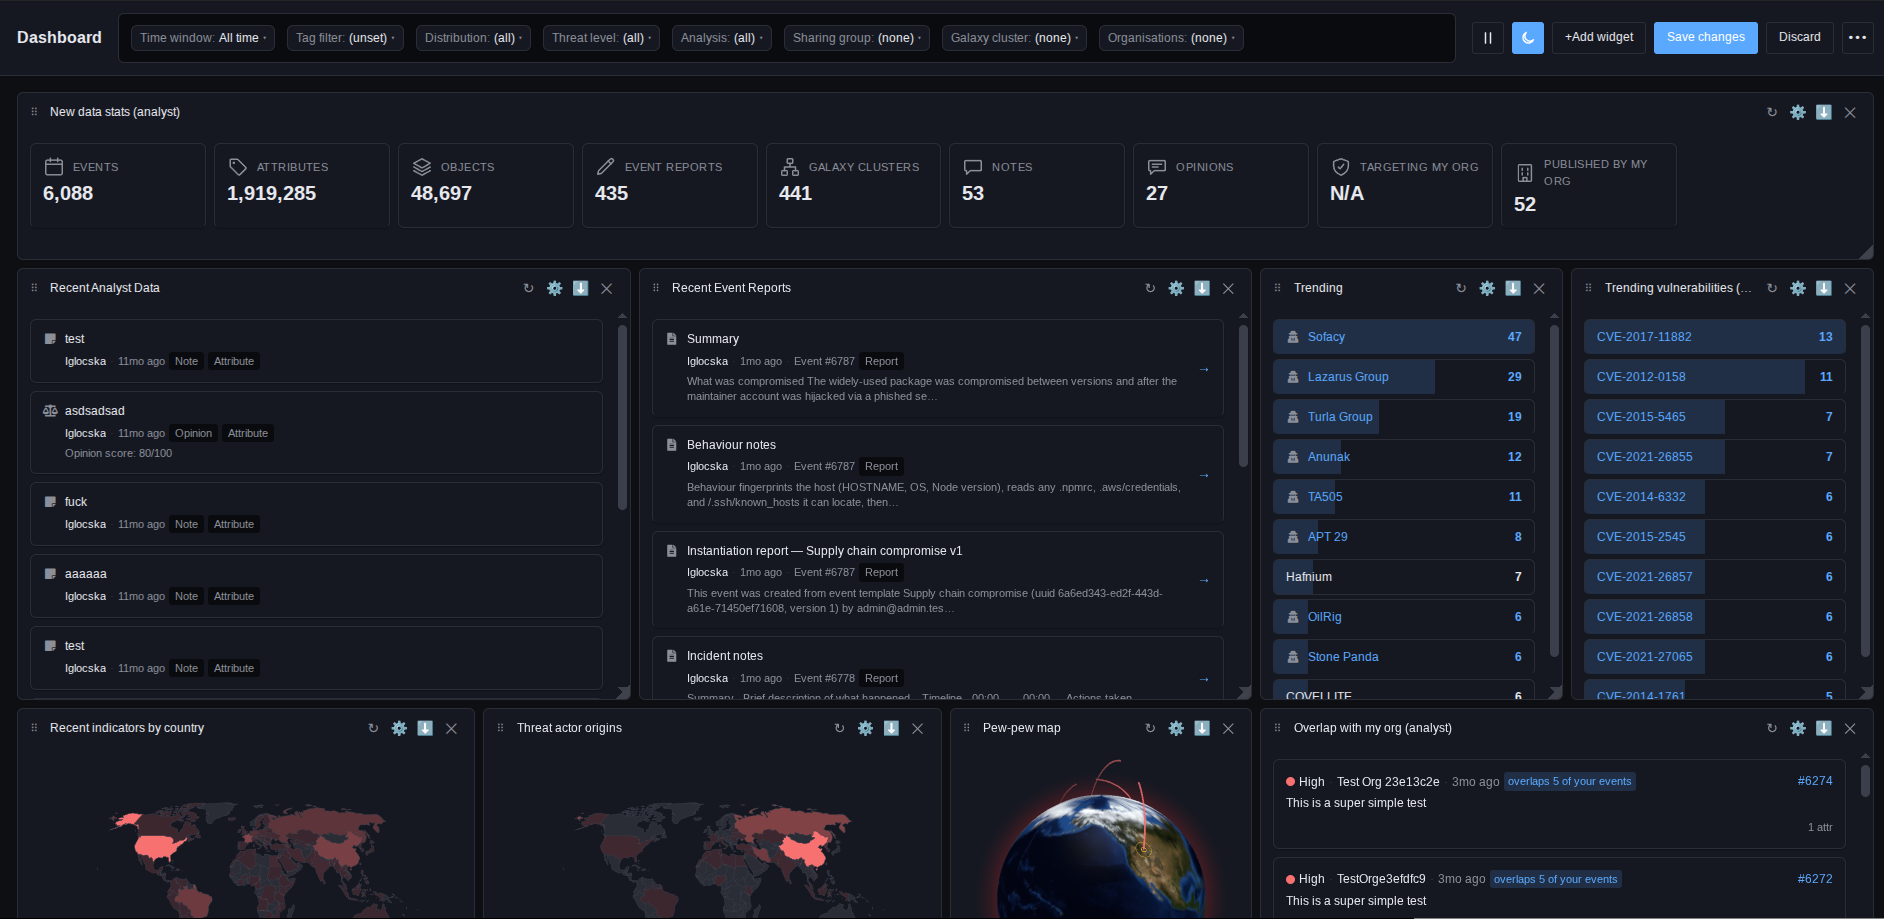
\includegraphics[width=\linewidth, keepaspectratio]{./img/misp-dashboard.png}

\end{frame}

\begin{frame}
    \frametitle{Event templating system}

    \begin{itemize}
        \item A {\bf total rewrite} of MISP's templating engine
        \item {\bf Drag-and-drop builder UI} with inline validation, object-template / taxonomy / galaxy pickers, and a live preview
        \item A {\bf Templates library} ships ten ready-to-use starter templates (ransomware, credential exposure, spearphishing, supply-chain, \dots)
        \item Migration helper for legacy templates, and full documentation
    \end{itemize}

\end{frame}

\begin{frame}
    \frametitle{New dashboard system: Templates Library \& Migration helper}
    \centering
    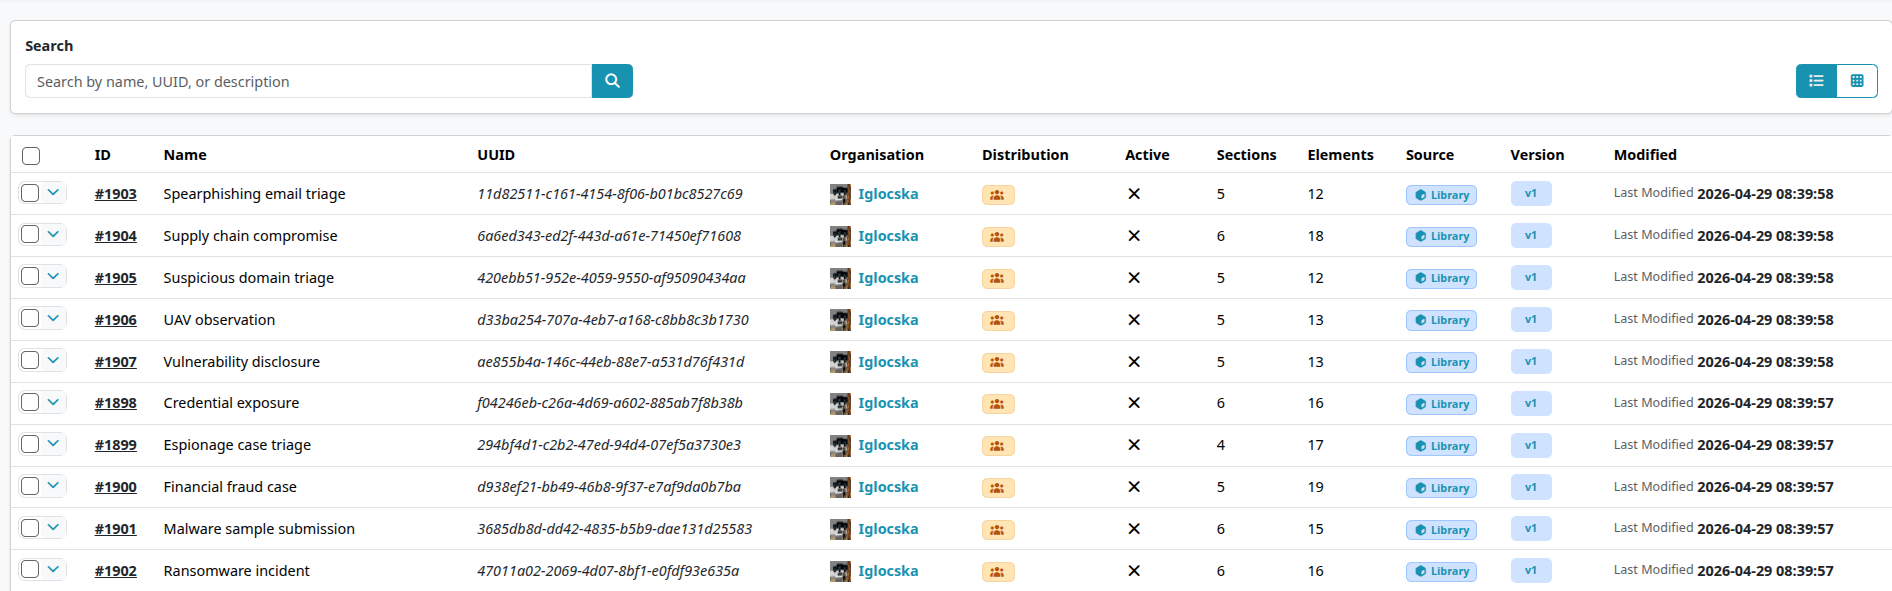
\includegraphics[width=1.0\linewidth, keepaspectratio]{./img/template-index.png}
\end{frame}

\begin{frame}
    \frametitle{New dashboard system: User form}
    \hspace*{-40pt}
    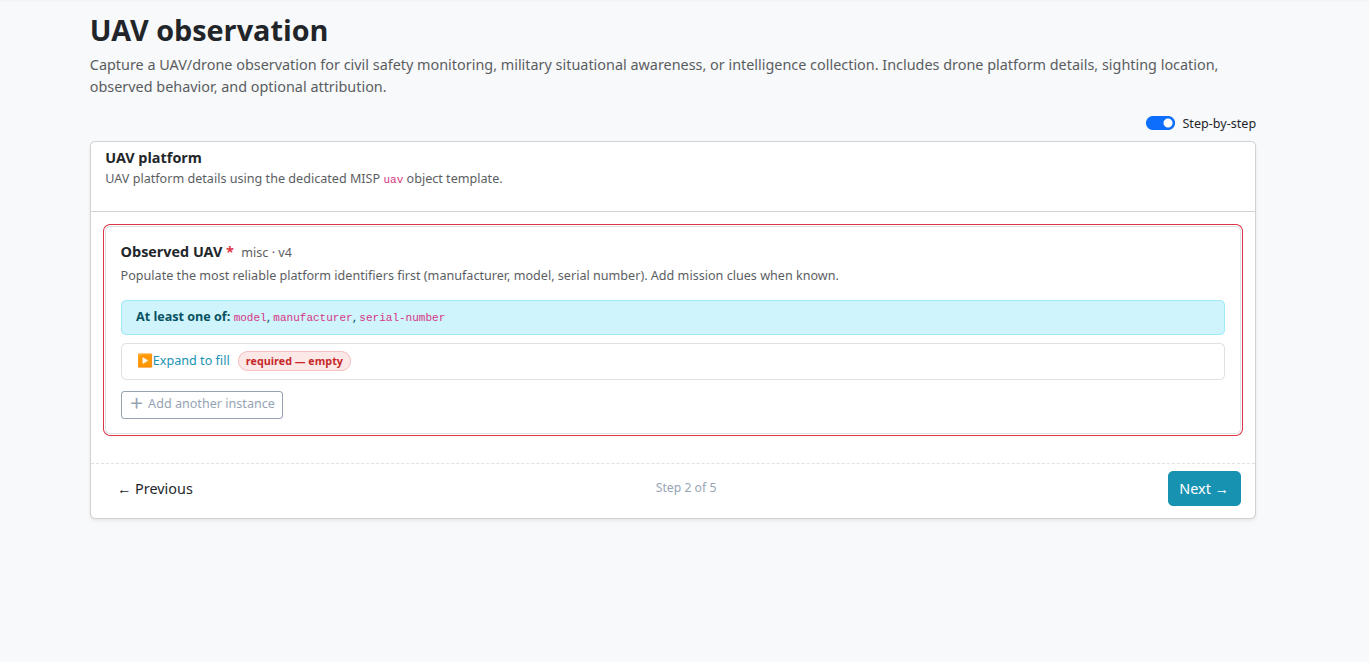
\includegraphics[width=1.2\linewidth, keepaspectratio]{./img/template-use.png}
\end{frame}

\begin{frame}
    \frametitle{New dashboard system: Builder UI}
    \centering
    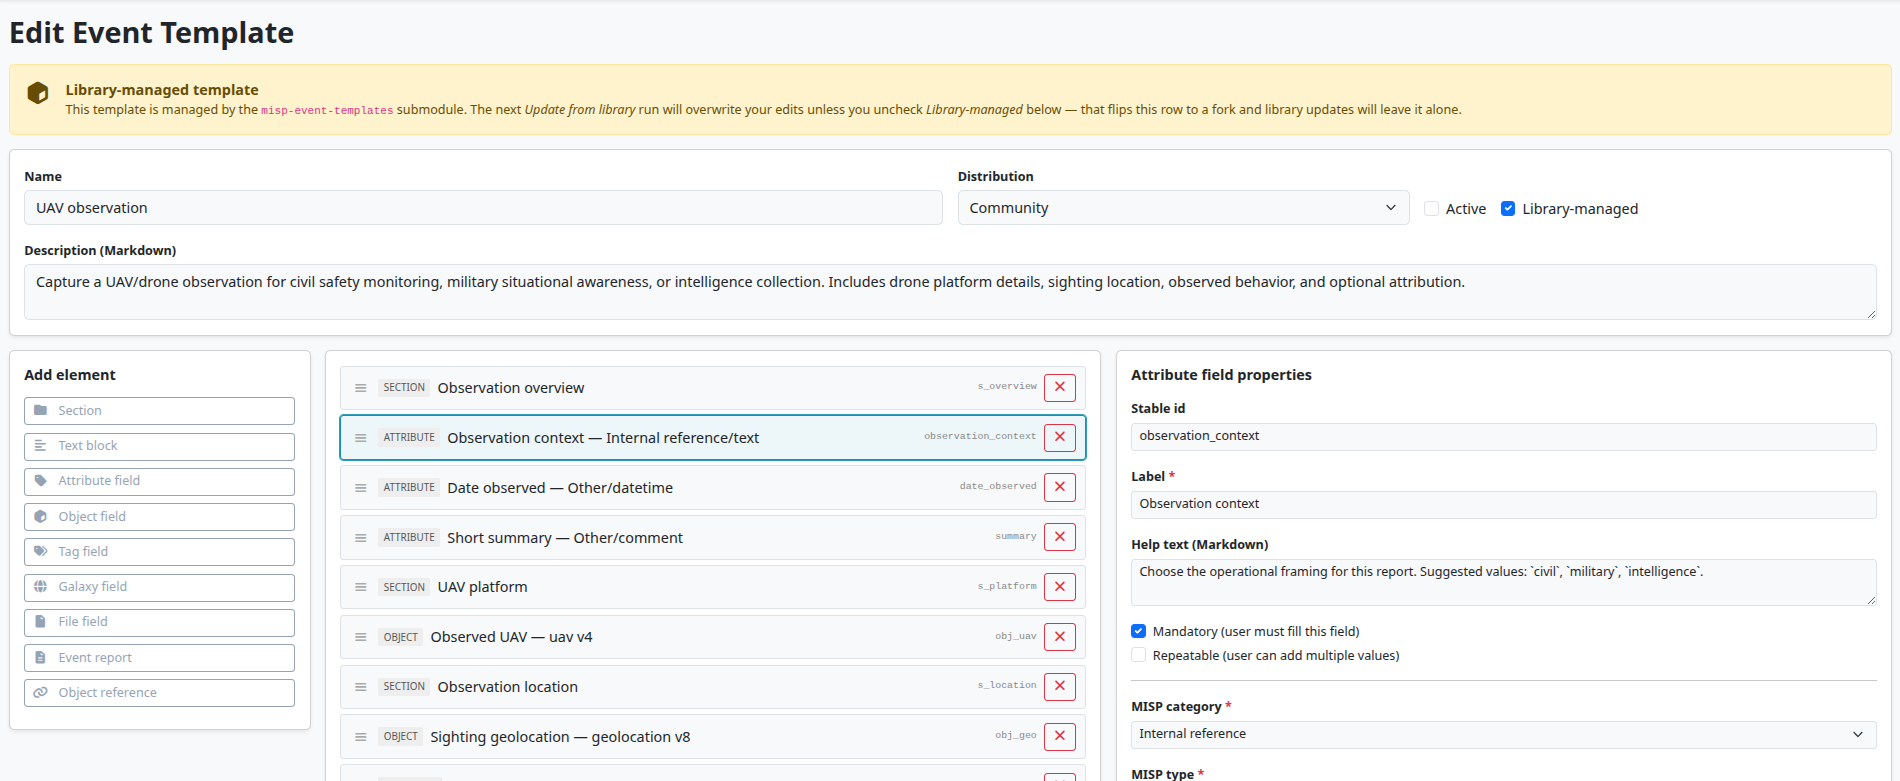
\includegraphics[width=1.0\linewidth, keepaspectratio]{./img/template-edit.png}
\end{frame}

\begin{frame}
    \frametitle{Geolocation \& map visualisation}

    \begin{itemize}
        \item Objects with geographic coordinates are now rendered on {\bf interactive tile-based maps}
        \item {\bf Accuracy-radius} visualisation
        \item Native {\bf GeoJSON} rendering for complex shapes and features
        \item {\bf GPX track} support for tracking objects
    \end{itemize}

    \alertbox{warning}{Disabled by default}{configurable tile server (defaults to \texttt{geo.circl.lu})}
\end{frame}

\begin{frame}
    \frametitle{Geolocation \& map visualisation}

    \begin{center}

    \begin{minipage}[t]{0.48\textwidth}
        \centering
        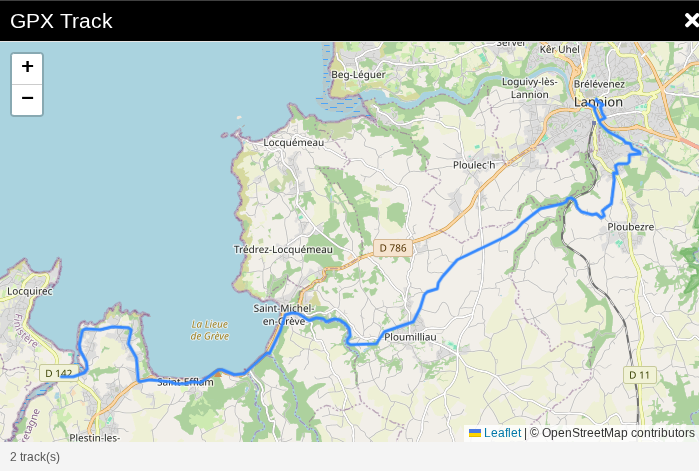
\includegraphics[width=\linewidth, keepaspectratio]{./img/gpx.png}

        \vspace{0.3em}
        \scriptsize \texttt{Full track}
    \end{minipage}
    \hfill
    \begin{minipage}[t]{0.48\textwidth}
        \centering
        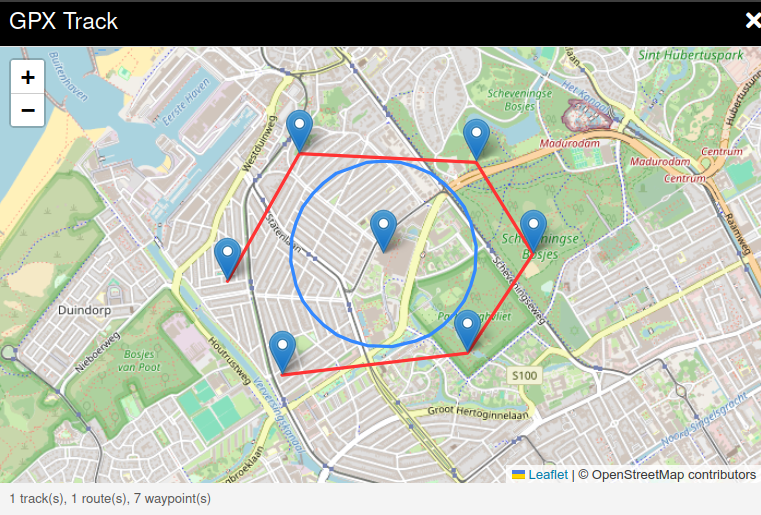
\includegraphics[width=\linewidth, keepaspectratio]{./img/gpx-europol.png}

        \vspace{0.1em}
        \scriptsize \texttt{Routes and waypoints}
    \end{minipage}

    \end{center}
\end{frame}
